\documentclass[titlepage = firstcover]{scrartcl}
\usepackage[aux]{rerunfilecheck}
\usepackage{fontspec}
\usepackage[main=ngerman, english, french]{babel}

% mehr Pakete hier
\usepackage{expl3}
\usepackage{xparse}

%Mathematik------------------------------------------------------
\usepackage{amsmath}   % unverzichtbare Mathe-Befehle
\usepackage{amssymb}   % viele Mathe-Symbole
\usepackage{mathtools} % Erweiterungen für amsmath
\usepackage[
  math-style=ISO,    % \
  bold-style=ISO,    % |
  sans-style=italic, % | ISO-Standard folgen
  nabla=upright,     % |
  partial=upright,   % /
]{unicode-math}% "Does exactly what it says on the tin."
\usepackage[section, below]{placeins}

% Laden von OTF-Mathefonts
% Ermöglich Unicode Eingabe von Zeichen: α statt \alpha

\setmathfont{Latin Modern Math}
%\setmathfont{Tex Gyre Pagella Math} % alternativ zu Latin Modern Math
\setmathfont{XITS Math}[range={scr, bfscr}]
\setmathfont{XITS Math}[range={cal, bfcal}, StylisticSet=1]

\AtBeginDocument{ % wird bei \begin{document}
  % werden sonst wieder von unicode-math überschrieben
  \RenewDocumentCommand \Re {} {\operatorname{Re}}
  \RenewDocumentCommand \Im {} {\operatorname{Im}}
}
\usepackage{mleftright}
\setlength{\delimitershortfall}{-1sp}

%Sprache----------------------------------------------------------
\usepackage{microtype}
\usepackage{xfrac}
\usepackage[autostyle]{csquotes}    % babel
\usepackage[unicode, pdfusetitle]{hyperref}
\usepackage{bookmark}
\usepackage[shortcuts]{extdash}
%Einstellungen hier, z.B. Fonts
\usepackage{booktabs} % Tabellen


\title{Wärmeleitfähigkeit}
\author{
  David Gutnikov\\
  \href{mailto:david.gutnikov@udo.edu}{david.gutnikov@udo.edu}
 \and 
  Lasse Sternemann\\
  \href{mailto:lasse.sternemann@udo.edu}{lasse.sternemann@udo.edu}
}
\date{Durchführung am 07.01.2020}


\begin{document}
  \maketitle
  \newpage
  \tableofcontents
  \newpage


\section{Auswertung}
    \subsection{Allgemeines}
        Im folgenden werden mehrfach Magnetfeldstärken bezüglich ihres Abstands zu einer der Spulenöffnungen angegeben. In diesen Fällen befindet sich die 
        Spulenöffnungen bei x=0. Negative Werte befinden sich außerhalb der Spule und positive Werte innerhalb, solange sie nicht die Länge der Spule 
        überschreiten. Der Wert magnetischen Feldkonstante $\mu_0$ wird in den Rechnungen aus der Konstantensammlung des National Institute of Standards 
        and Technology [2] entnommen.
    \subsection{Magnetfelder in einfachen Spulen}
        \subsubsection{Magnetfeld einer langen Spule}
            Um einen Vergleichswert zur Magnetfeldstärke in der langen Spule zu haben, wird über Formel xxx ein Theoriewert berechnet. Dazu werden folgende 
            Eigenschaften der Spule und Experimentierbedigungen verwendet:
            \begin{equation*}  
                L = 0,155m \qquad N = 300 \qquad I = 0,68 A 
            \end{equation*}    
            Somit ergibt sich für das homogene Magnetfeld innerhalb der langen Spule der Referenzwert:
            \begin{equation}
                B = 1,65 mT 
                \label{eqn:BLang}
            \end{equation}
            Dieser wird mit den in Abbildung \ref{fig:Spulelang} dargestellten und in Tabelle \ref{tab:Spulelang} eingetragenen Messwerten verglichen.

            \begin{table}[h]
                \centering 
                \caption{In der Tabelle ist die Stärke des Magnetfelds in Abhängigkeit von der Distanz zu einer der Spulenöffnung aufgelistet.}
                \label{tab:Spulelang}

                \begin{tabular}{c c c c}
                    \toprule
                    {x \ [m]} & {B \ [mT]} & {x \ [m]} & {B \ [mT]} \\
                    \midrule
                    -0,04 & 0,088  &  0,08   & 1,574 \\
                    -0,03 & 0,128  &  0,09   & 1,566 \\
                    -0,02 & 0,208  &  0,10   & 1,552 \\
                    -0,01 & 0,377  &  0,11   & 1,483 \\
                    0     & 0,69   &  0,12   & 1,483 \\
                    0,01  & 1,08   &  0,13   & 1,397 \\
                    0,02  & 1,322  &  0,14   & 1,217 \\
                    0,03  & 1,443  &  0,15   & 0,879 \\
                    0,04  & 1,506  &  0,16   & 0,502 \\
                    0,05  & 1,538  &  0,17   & 0,272 \\
                    0,06  & 1,559  &  0,18   & 0,158 \\
                    0,07  & 1,569  &         & \\
                    \bottomrule
                \end{tabular}                
            \end{table}

            \begin{figure}[h]
                \centering
                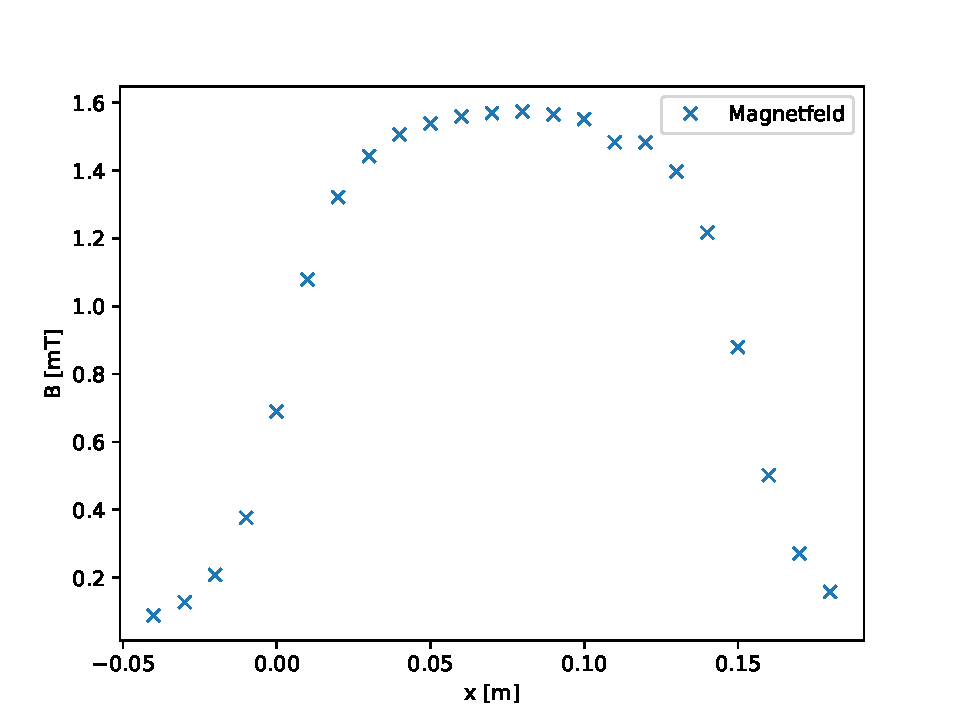
\includegraphics{Spulelang.pdf}
                \caption{In dieser Abbildung sind die Werte aus der obrigen Tabelle aufgetragen. Sie zeigen das Magnetfeld abhängig von der Entfernung zur Spulenöffnung, die bei x=0 liegt.}
                \label{fig:Spulelang}

            \end{figure}

            \FloatBarrier
            \newpage


        \subsubsection{Magnetfeld einer kurzen Spule}
            Auch bei der kurzen Spule wird zuerst über Formel xxx ein theoretischer Referenzwert berechnet.
            \begin{align*}
                L = 0,09cm \qquad N = 3400 \qquad I = 0,08A 
            \end{align*}
            \begin{equation}
                B = 3,80 mT \\
                \label{eqn:Bkurz}
            \end{equation} 
            Dieser wird später mit den Messwerten aus Tabelle \ref{tab:Spulekurz} verglichen. Der Verlauf dieser Messwerte ist auch in Abbildung 
            \ref{fig:Spulekurz} dargestellt.
            \begin{table}[h]
                \centering 
                \caption{In der Tabelle ist die Stärke des Magnetfelds in Abhängigkeit von der Distanz zu einer der Spulenöffnung aufgelistet.}
                \label{tab:Spulekurz}

                \begin{tabular}{c c c c}
                    \toprule
                    {x \ [m]} & {B \ [mT]} \\
                    \midrule
                    -0,04 & 0,602 \\
                    -0,03 & 0,777 \\
                    -0,02 & 0,995 \\
                    -0,01 & 1,271 \\
                     0,00 & 1,579 \\
                     0,01 & 1,885 \\
                     0,02 & 2,165 \\
                     0,03 & 2,375 \\
                     0,04 & 2,5   \\
                     0,05 & 2,529 \\
                     0,06 & 2,462 \\
                     0,07 & 2,299 \\
                     0,08 & 2,052 \\
                     0,09 & 1,761 \\
                     0,1  & 1,444 \\
                     0,11 & 1,142 \\
                    \bottomrule
                \end{tabular}                
            \end{table}

            \begin{figure}[h]
                \centering
                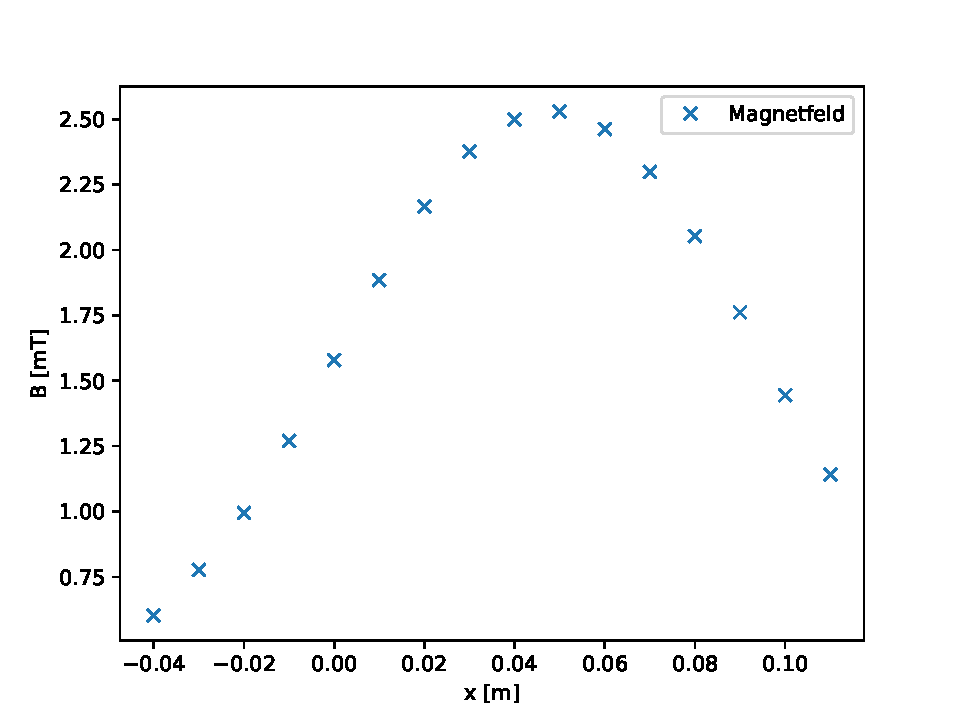
\includegraphics{Spulekurz.pdf}
                \caption{In dieser Abbildung sind die Werte aus der obrigen Tabelle aufgetragen. Sie zeigen das Magnetfeld abhängig von der Entfernung zur Spulenöffnung, die bei x=0 liegt.}
                \label{fig:Spulekurz}

            \end{figure}

            \FloatBarrier
            \newpage


    \subsection{Magnetfelder von Helmholtzspulen}
            Bei den folgenden Helmholtzspulenpaaren wurde nur der Spulenabstand varriert, demnach haben sie ansonsten die gleichen Eigenschaften und wurden an
            die gleiche Stromstärke angeschlossen.
            \begin{equation*}
                R = 0,0625m \qquad N = 100 \qquad I = 1,94A \\
            \end{equation*}
            \subsubsection{Spulenabstand 10cm}
            Bei diesem Spulenpaar beträgt der Spulenabstand 0,1m. Mit diesem und den allgemeinen Werten, die für alle Helmholtzspulenpaare gelten, lässt sich
            folgender Referenzwert für die Mitte zwischen den zwei Spulen, die bei 5cm liegt, berechnen.
            \begin{equation}
                B_{\text{Mitte}} = 1,86 mT\\
                \label{eqn:HelmA}
            \end{equation}
            Die gemessenen Magnetfeldstärken \ref{tab:HelmholtzA} werden in Abbildung \ref{fig:HelmholtzA} gegen den Abstand zur Spule angegeben.
            \begin{table}[h]
                \centering 
                \caption{In der Tabelle ist die Stärke des Magnetfelds in Abhängigkeit von der Distanz zu einer der Spulenöffnung aufgelistet.}
                \label{tab:HelmholtzA}

                \begin{tabular}{c c c c}
                    \toprule
                    {x \ [m]} & {B \ [mT]} & {x \ [m]} & {B \ [mT]} \\
                    \midrule
                    0,01  & 2,01  & 0,12 & 1,267 \\
                    0,015 & 1,968 & 0,13 & 1,034 \\
                    0,02  & 1,947 & 0,14 & 0,837 \\
                    0,025 & 1,929 & 0,15 & 0,674 \\
                    0,03  & 1,934 & 0,16 & 0,547 \\
                    0,035 & 1,943 & 0,17 & 0,444 \\
                    0,04  & 1,973 & 0,18 & 0,362 \\
                    0,045 & 2,006 & 0,19 & 0,298 \\
                    0,05  & 2,051 & 0,20 & 0,245 \\
                    0,11  & 1,526 & & \\
                    \bottomrule
                \end{tabular}                
            \end{table}

            \begin{figure}[h]
                \centering
                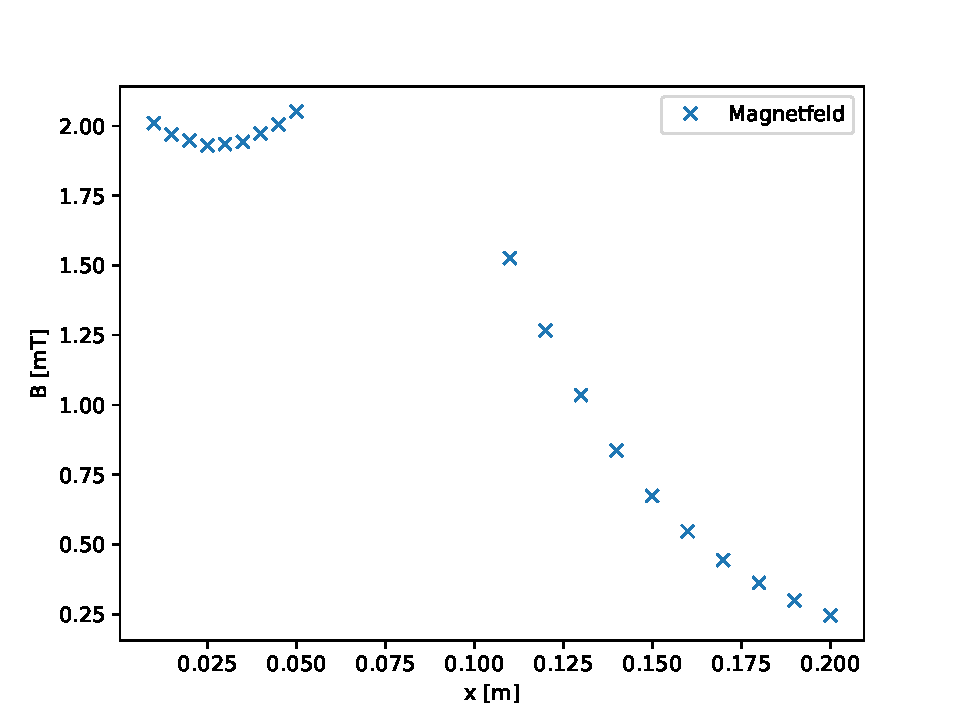
\includegraphics{HelmholtzA.pdf}
                \caption{In dieser Abbildung sind die Werte aus der obrigen Tabelle aufgetragen. Sie zeigen das Magnetfeld abhängig von der Entfernung zur Spulenöffnung, die bei x=0 liegt.}
                \label{fig:HelmholtzA}

            \end{figure}

            \FloatBarrier
            \newpage

            \subsubsection{Spulenabstand 15cm}
            Hier wird die Magnetfeldstärke im Mittelpunkt, der bei 7,075,5cm liegt, analog zur ersten Helmholtzspule berechnet. Der Spulenabstand beträgt nun 
            jedoch 0,15m. Die Werte finden sich in Tabelle \ref{tab:HelmholtzB} und der Verlauf der Magnetfeldstärke in Abbildung \ref{fig:HelmholtzB}.
            \begin{equation}
                B_{\text{Mitte}} = 1,02mT \\
                \label{eqn:HelmB}
            \end{equation}
            \begin{table}[h]
                \centering 
                \caption{In der Tabelle ist die Stärke des Magnetfelds in Abhängigkeit von der Distanz zu einer der Spulenöffnung aufgelistet.}
                \label{tab:HelmholtzB}

                \begin{tabular}{c c c c}
                    \toprule
                    {x \ [m]} & {B \ [mT]} & {x \ [m]} & {B \ [mT]} \\
                    \midrule
                    0,01  & 1,579 & 0,07 & 1,207 \\
                    0,02  & 1,403 & 0,075 & 1,245 \\
                    0,03  & 1,261 & 0,08 & 1,329 \\
                    0,035 & 1,207 & 0,09 & 1,489 \\
                    0,04  & 1,165 & 0,10 & 1,670 \\
                    0,045 & 1,131 & 0,16 & 1,420 \\
                    0,05  & 1,123 & 0,17 & 1,173 \\
                    0,055 & 1,113 & 0,18 & 0,959 \\
                    0,06  & 1,137 & 0,19 & 0,770 \\
                    0,065 & 1,152 & 0,20 & 0,618 \\
                    \bottomrule
                \end{tabular}                
            \end{table}

            \begin{figure}[h]
                \centering
                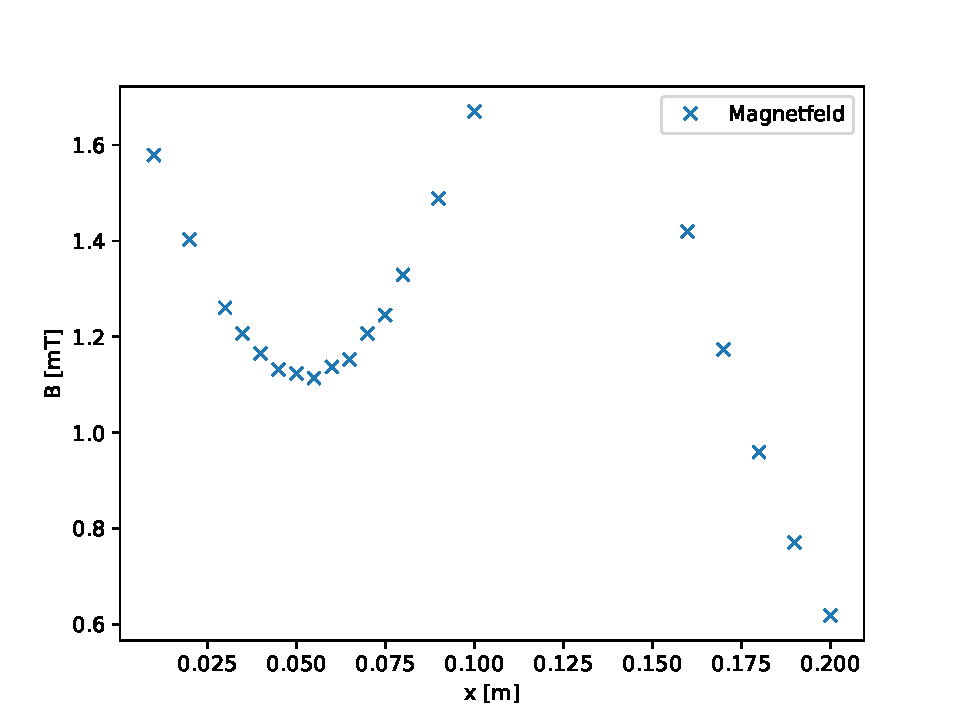
\includegraphics{HelmholtzB.pdf}
                \caption{In dieser Abbildung sind die Werte aus der obrigen Tabelle aufgetragen. Sie zeigen das Magnetfeld abhängig von der Entfernung zur Spulenöffnung, die bei x=0 liegt.}
                \label{fig:HelmholtzB}

            \end{figure}

            \FloatBarrier
            \newpage

            \subsubsection{Spulenabstand 20cm}
            Nun beträgt der Spulenabstand 0,2m und die Berechnung erfolgt wieder analog zu den anderen Rechnungen.
            \begin{equation}
                B_{\text{Mitte}} = 0,58 mT \\
                \label{eqn:HelmC}
            \end{equation} 
            Der Verlauf der in Tabelle \ref{tab:HelmholtzC} gegebenen Magnetfeldstärken wird in Abbildung \ref{fig:HelmholtzC} dargestellt. 
            \begin{table}[h]
                \centering 
                \caption{In der Tabelle ist die Stärke des Magnetfelds in Abhängigkeit von der Distanz zu einer der Spulenöffnung aufgelistet.}
                \label{tab:HelmholtzC}

                \begin{tabular}{c c c c}
                    \toprule
                    {x \ [m]} & {B \ [mT]} & {x \ [m]} & {B \ [mT]} \\
                    \midrule
                    0,01 & 1,458 & 0,11 & 0,832 \\
                    0,02 & 1,250 & 0,12 & 0,965 \\
                    0,03 & 1,058 & 0,13 & 1,131 \\
                    0,04 & 0,906 & 0,14 & 1,330 \\
                    0,05 & 0,791 & 0,15 & 1,534 \\
                    0,06 & 0,714 & 0,21 & 1,366 \\
                    0,07 & 0,672 & 0,22 & 1,135 \\
                    0,08 & 0,661 & 0,23 & 0,917 \\
                    0,09 & 0,684 & 0,24 & 0,737 \\
                    0,10 & 0,742 & 0,25 & 0,585 \\
                    \bottomrule
                \end{tabular}                
            \end{table}

            \begin{figure}[h]
                \centering
                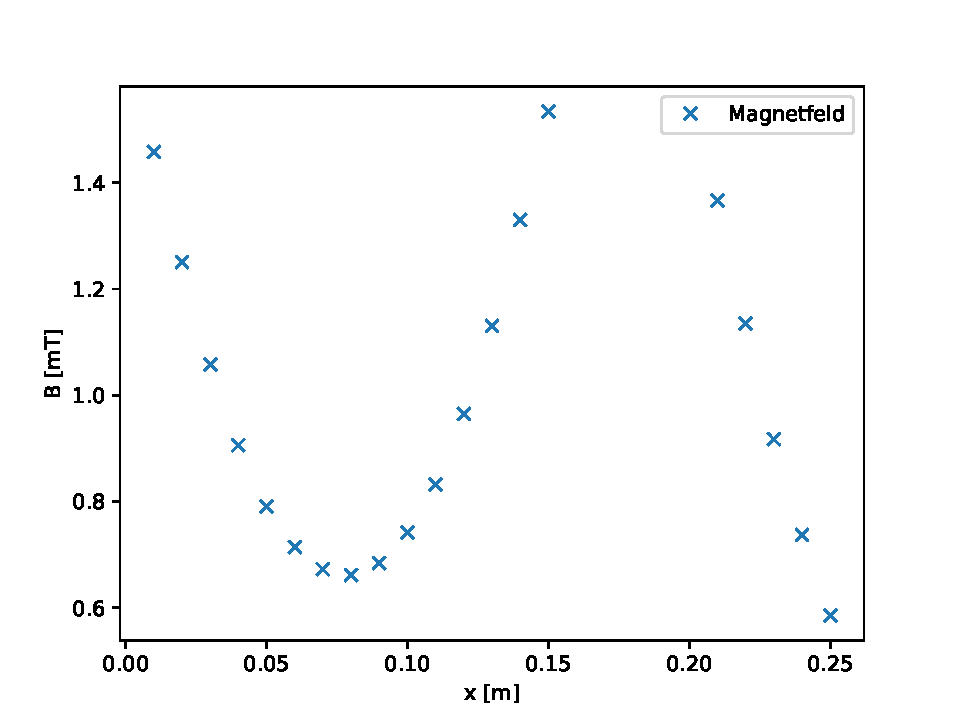
\includegraphics{HelmholtzC.pdf}
                \caption{In dieser Abbildung sind die Werte aus der obrigen Tabelle aufgetragen. Sie zeigen das Magnetfeld abhängig von der Entfernung zur Spulenöffnung, die bei x=0 liegt.}
                \label{fig:HelmholtzC}

            \end{figure}

            \FloatBarrier
            \newpage
                
        \subsection{Hysteresekurve}
            Die durch Auftragen der in Tabelle \ref{tab:Hysterese} eingetragenen Werte wird die Hysteresekurve \ref{fig:Hysterese} modelliert. Sie beinhaltet 
            5 gesonderte Werte. Die Remanenz, die die Magnetfeldstärke bei nicht vorhandener Stromstärke angibt.
            \begin{align}
                B_{\text{R1}} = 131 \; A \\
                B_{\text{R2}} = -133 \; A 
                \label{eqn:Remanenzen}
            \end{align}
            Die zwei anderen ausgezeichneten Werte beschreiben die Koerzitivkraft, die dem gegebenen magnetischen Feld so entgegenwirkt, dass die gesamte
            Magnetfeldstärke null ist. Diese Punkte liegen bei folgenden Stromstärken.
            \begin{align}
                I_{\text{C1}} = -0,65 \; A\\
                I_{\text{C2}} = 0,68 \; A
                \label{eqn:Koerzitiv}
            \end{align} 
            Der letzte Wert ist die Sättigungsmagnetisierung, die bei uns wiefolgt gemessen wurde:
            \begin{equation*}
                B_{\text{Sättigung}} = 726 \; mT
            \end{equation*}
        \begin{table}[h]
            \centering 
            \caption{In der Tabelle ist die Stärke des Magnetfelds in Abhängigkeit von der Distanz zu einer der Spulenöffnung aufgelistet.}
            \label{tab:Hysterese}

            \begin{tabular}{c c c c}
                \toprule
                {x \ [m]} & {B \ [mT]} & {x \ [m]} & {B \ [mT]} \\
                \midrule
                0 & 2,7   & -6   & -599 \\
                1 & 149   & -7   & -640 \\
                2 & 350   & -8   & -672 \\
                3 & 446   & -9   & -702 \\
                4 & 508   & -10  & -730 \\
                5 & 560   & -9   & -711 \\
                6 & 605   & -8   & -693 \\
                7 & 640   & -7   & -671 \\
                8 & 670   & -6   & -645 \\
                9 & 700   & -5   & -617 \\
                10 & 726  & -4   & -580 \\
                9 & 709   & -3   & -533 \\
                8 & 691   & -2   & -467 \\
                7 & 668   & -1   & -331 \\
                6 & 644   &  0   & -133 \\
                5 & 614   & 0,68 &    0 \\
                4 & 576   & 1    &   81 \\
                3 & 520   & 2    &  258 \\
                2 & 464   & 3    &  391 \\
                1 & 327   & 4    &  489 \\
                0 & 131   & 5    &  549 \\
                -0,65 & 0 & 6    &  595 \\
                -1 & -70  & 7    &  638 \\
                -2 & -256 & 8    &  696 \\
                -3 & -392 & 9    &  699 \\
                -4 & -490 & 10   &  725 \\
                -5 & -552 & & \\
                \bottomrule
            \end{tabular}                
        \end{table}

        \begin{figure}[h]
            \centering
            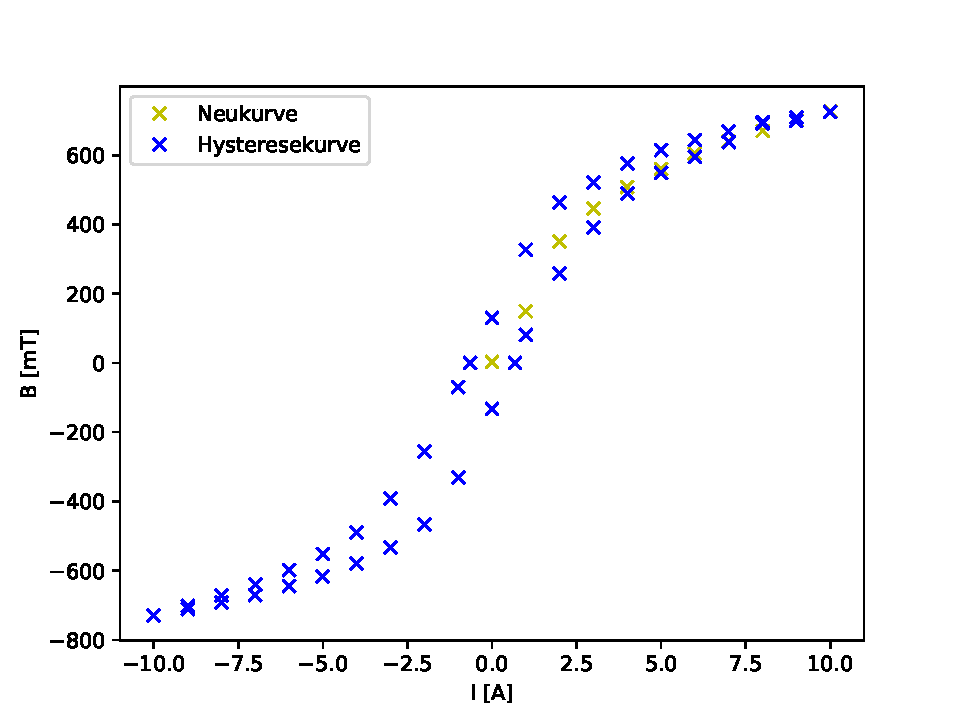
\includegraphics{Hysterese.pdf}
            \caption{In dieser Abbildung sind die Magnetfeldstärke gegen die Stromstärken aufgetragen, sodass sich die Hysteresekurve ergibt.}
            \label{fig:Hysterese}

        \end{figure}

        \newpage
        
\section{Diskussion}
        Zur Verifizierung der Messreihen werden die Theoriewerte mit den gemessenen Werten verglichen. Bei den beiden normalen Spulen wird der Theoriewert mit
        dem Wert in der Mitte der Spule verglichen. So weicht die Magnetfeldstärke der langen Spule, $B_{\text{Messung}} = 1,574 mT$,  um 4,81 \% von dem errechneten Wert 
        \ref{eqn:BLang} ab. Der Wert der kurzen Spule, $B_{\text{Messung}} = 2,529 mT$, weicht um 43,45 \% vom Theoriewert \ref{eqn:Bkurz} ab. Während der Wert
        der langen Spule gut mit dem Theoriewert übereinstimmt, weicht der der kurzen Spule stärker von dessen Theoriewert ab. Dies liegt vermutlich an der 
        Annahme, dass die kurze Spule die Bedingungen für die Annäherung einer langen Spule nicht genügend erfüllt. Die lange Spule hingegen erfüllt die 
        Bedingung hinreichend und die Abweichung zum Theoriewert fällt dementsprechend gering aus. Quantitativ liefern 
        beide Kurven das erwartete Ergebnis. Die lange Spule weist ein Plataeu auf, das bei der kurzen Kurve verschwindet und nur noch als Peak zu sehen ist.
        Bei den Helmholtzspulenpaaren werden die theoretischen Werte mit den gemessenen Werten in den Zentren der Helmholtzspulenpaaren verglichen.
        \begin{align*}
            10cm \qquad B_{\text{Messung}} = 2,051 mT \qquad B_{\text{Theorie}} = 1,86 mT \qquad \text{Abweichung}: \; 9,31 \% \\
            15cm \qquad B_{\text{Messung}} = 1,245 mT \qquad B_{\text{Theorie}} = 1,02 mT \qquad \text{Abweichung}: \; 17,83 \% \\
            20cm \qquad B_{\text{Messung}} = 0,742 mT \qquad B_{\text{Theorie}} = 0,58 mT \qquad \text{Abweichung}: \; 21,83 \% 
        \end{align*}
        Unter Rücksichtnahme auf die äußeren Faktoren wie die Magnetfelder der anderen Gruppenexperimente bestätigen auch diese Theoriewerte die Messung.
        Unterstützt wird dies durch die erwartete Form der Plots in den Graphen \ref{fig:HelmholtzA}, \ref{fig:HelmholtzB} und \ref{fig:HelmholtzC}. Die Feld-
        stärke wird zu den Spulen maximal und sinkt gegen das Zentrum. Wie zu erwarten sinkt die Kurve stärker bei größeren Spulenabständen.
        Die letzte Messung liefer die Hysteresekurve, welche ebenfalls der erwarteten Form entspricht. Auch die zu erwartende Symmetrie lässt sich durch die 
        Ähnlichkeit der Remanenzen \ref{eqn:Remanenzen}, die um 1,5 \% voneinander abweichen und die Ähnlichkeit der Koerzitivstromstärken \ref{eqn:Koerzitiv},
        die um 4,41 \% voneinander abweichen. 

\newpage
\section{Literaturverzeichnis}
        [1] \textit{Versuchsanleitung V308 - Magnetfelder und Spulen.} TU Dortmund, 2019 \newline
        [2] National Institute of Standards and Technology: \textit{Fundamental Physical Constants} 09.Dezember.2019
            \url{https://physics.nist.gov/cgi-bin/cuu/Value?r}
\end{document}